\chapter{High Purity Germanium Detectors}
\label{chap:detectors}

\section{Introduction}
${}^{76}Ge$ double-beta decays into ${}^{76}Se$, represented by the equation \ref{germanium_0nbb_eq}. It has several advantages as a source for $0\nu\beta\beta$ decay experiments. As a semi-conductor, it can be made into detectors with excellent energy resolution, which is critical as energy is the only observable that is both necessary and sufficient for a discovery. Its Q value is $2.039$ MeV, which is above the energies of most gamma events. The crystal-growing process for Germanium has purification stages that can highly reduce internal backgrounds such as $^{238}$U and $^{232}$Th chain contaminants. Germanium is abundant in nature and can be easily enriched, allowing for large-scale experiments. Signal formation inside Germanium is well understood and enables precise topology-based discrimination between background and signal events through pulse shape discrimination (PSD) techniques. Germanium detectors thus have an extensive history in nuclear physics and rare-event searches.


\begin{equation}\label{germanium_0nbb_eq}
{}_{32}^{76}Ge \rightarrow {}_{34}^{76}Se + 2e^- + 2\bar{\nu}_e
\end{equation}

Fig. ~\ref{past_ge_exp} shows a past timeline of Ge-based experiments. Over the years, research and development have resulted in experiments that continuously provide a larger bound to the half-life of the reaction while reducing the background. The MAJORANA and GERDA collaborations are two such experiments with extensive experience in the research and development of Germanium detectors.

\begin{figure}[!htb]
\centering
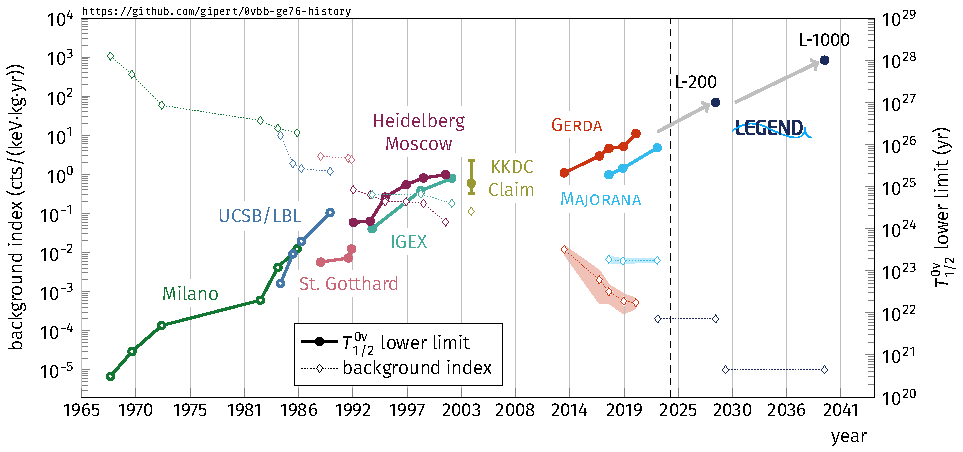
\includegraphics[trim=0.1cm 0 0.1cm 0,clip, width=0.99\linewidth]{ch2/figs/0nbb-ge76-history-future.pdf}
\caption{A plot showing a timeline of past and future Germanium-based $o\nu\beta\beta$ decay experiments. The the half-lives probed by them is shown along with their background index. Next generation experiments aim to continue improve half life limit while having the lowest background index. Plot credit: Luigi Pertoldi}
\label{past_ge_exp}
\end{figure}


\section{Signal formation in Germanium}
\subsection{Germanium properties}
The lattice structure of crystalline metals results in allowed energy bands for the electrons. The outermost bound state is termed the valence band, and the unbound state, the conduction band. The difference between the valence and minimal conduction band energy is called the band gap. Electrons of all lattice atoms can move freely in the conduction band. In metals, the band gap is non-existent, with the valence and conduction bands overlapping, which makes metals very good conductors. In insulators, the band gap is large, which makes them poor electric conductors.

In semiconductors, the band gap is intermediate ($2.96$ eV for Ge) which makes it possible to use semiconductor crystals as a radiation detector. Due to the ideal band gap, radiation excites multiple electrons to the conduction band, leaving behind a positively charged atom (hole). Both charge carriers can drift along the electric field and can be measured at a readout electrode. In reality, the holes do not drift. An electron from an adjacent atom fills the hole, and another electron fills the new hole, and the process continues until the last hole is filled by the cathode. The process gives an illusion that the hole is drifting towards the negative terminal, and we will treat it as such.

\subsection{P-type Point Contact Germanium Detectors}
A Germanium-based detector would measure the total energy deposited by collecting charge carriers at the readout electrodes. This is achieved by applying an external electric field to drift the charges towards the electrodes. There is still a steady `leakage' current due to the thermal excitation of electrons. To reduce the leakage current, detectors are operated at low temperatures, but low electric fields make it difficult to efficiently detect radiation with just pure Germanium. Impurities are added to improve detector performance.

The impurities come in two forms: electron donors and receivers. Donors provide excess loosely-bound electrons in the semiconductor and are called n-type, while the receivers increase the net number of holes and are called p-type. Impurities can be intentionally added to semiconductors to control the charge carrier and increase the conductivity by a process called doping. For example, doping Germanium with a group $15$ element such as Arsenic will make it n-type as Arsenic has 5 valence electrons compared to four in Germanium. Similarly, doping Germanium with a group 13 element such as Aluminum (3 valence electrons) would make it p-type.

While manufacturing a high purity Germanium crystal, the impurities are added to a molten bath and the crystal is pulled via the Czochralski method. The concentration of impurities is not uniform throughout the crystal. In Germanium, this depends on the solubility ratio of the impurities in the solid and liquid phases, known as the segregation coefficient. A segregation coefficient close to $1$ such as for Aluminum will result in it being uniformly distributed in the crystal. For several n-type impurities like phosphorous and oxygen, the segregation coefficient is less than 1, and the impurities would prefer to be in a liquid state. As the crystal is pulled from its melt, the impurities with low segregation coefficients prefer the liquid phase and get concentrated in the bath. This will result in the tail having a higher impurity concentration. The net effect is an impurity gradient, which is important to consider while simulating signal formation inside the detector.

A diode is when a p-type semiconductor is joined with an n-type semiconductor. The excess charges diffuse into each other, creating a region with no free charge carriers called the depletion region. The process produces a net positive charge on the n side of the material and an equal-magnitude negative charge on the p side. It results in a potential difference across the material, termed the contact potential. If an external potential is applied opposite to the contact potential (positive potential on the p side, termed forward bias), there will be a free flow of current; however, if the external potential difference is applied opposite to the contact potential (positive potential on the n side, termed reverse bias), more charge carriers will diffuse, resulting in a bigger depletion region and lower leakage current. This depletion region is ideal for detecting incident radiation as the charges excited by the radiation are immediately collected and read by the electrodes.

The depletion region can be measured by the detector's capacitance. The capacitance will keep decreasing until a certain potential, called the depletion voltage, is reached. Depletion voltage is where the biggest possible depletion region is achieved. It has been known that reducing the overall capacitance of HPGe detectors would decrease noise and increase energy resolution. This can be achieved by using a point-like central contact for the electrodes. In general, holes are less sensitive to charge trapping, and thus P-type detectors are preferred over N-type detectors for point-contact detector geometries.

\subsection{Shockley-Ramo Theorem}
Energy deposition in the detector will create charge clouds of electrons and holes. These charges induce an image charge on the point contact which is kept at zero potential. As these charge clouds drift under the external electric field, the image charges also drift, inducing a current at the point contact. The electrons and holes drift in opposite directions and result in a net positive induced signal on the read-out electrode. The Shockley–Ramo theorem gives the induced charge $Q(t)$ on an electrode caused by a moving charge $q$:

\begin{equation}\label{wp_eq}
Q(t)=q\Delta \phi_0(t)
\end{equation}

The weighting potential $\phi_0(t)$ is the solution of the Laplace equation with the boundary conditions of $\phi_0=1$ for the readout electrode and $\phi_0=0$ for all other electrodes. Fig. \ref{fig:wp_signal} left shows the calculated weighing potential inside a point contact detector used in {\MJD}. Note that the weighing potential is close to zero for most of the bulk. Thus, most energy depositions create charge clouds in the detector region with low weighting potential. Holes end up traveling a bigger change in potential than electrons since the point contact has a weighting potential of $1$. This bigger change means that hole contribution dominates the signal. Holes encounter most of this potential difference in the region near point contact, which results in a step-shaped signal shown by a sample waveform from a ${}^{76}Ge$ detector in Fig. \ref{fig:wp_signal}.

  \begin{figure}[htb]
  \centering
   %[trim={left bottom right top},clip]
  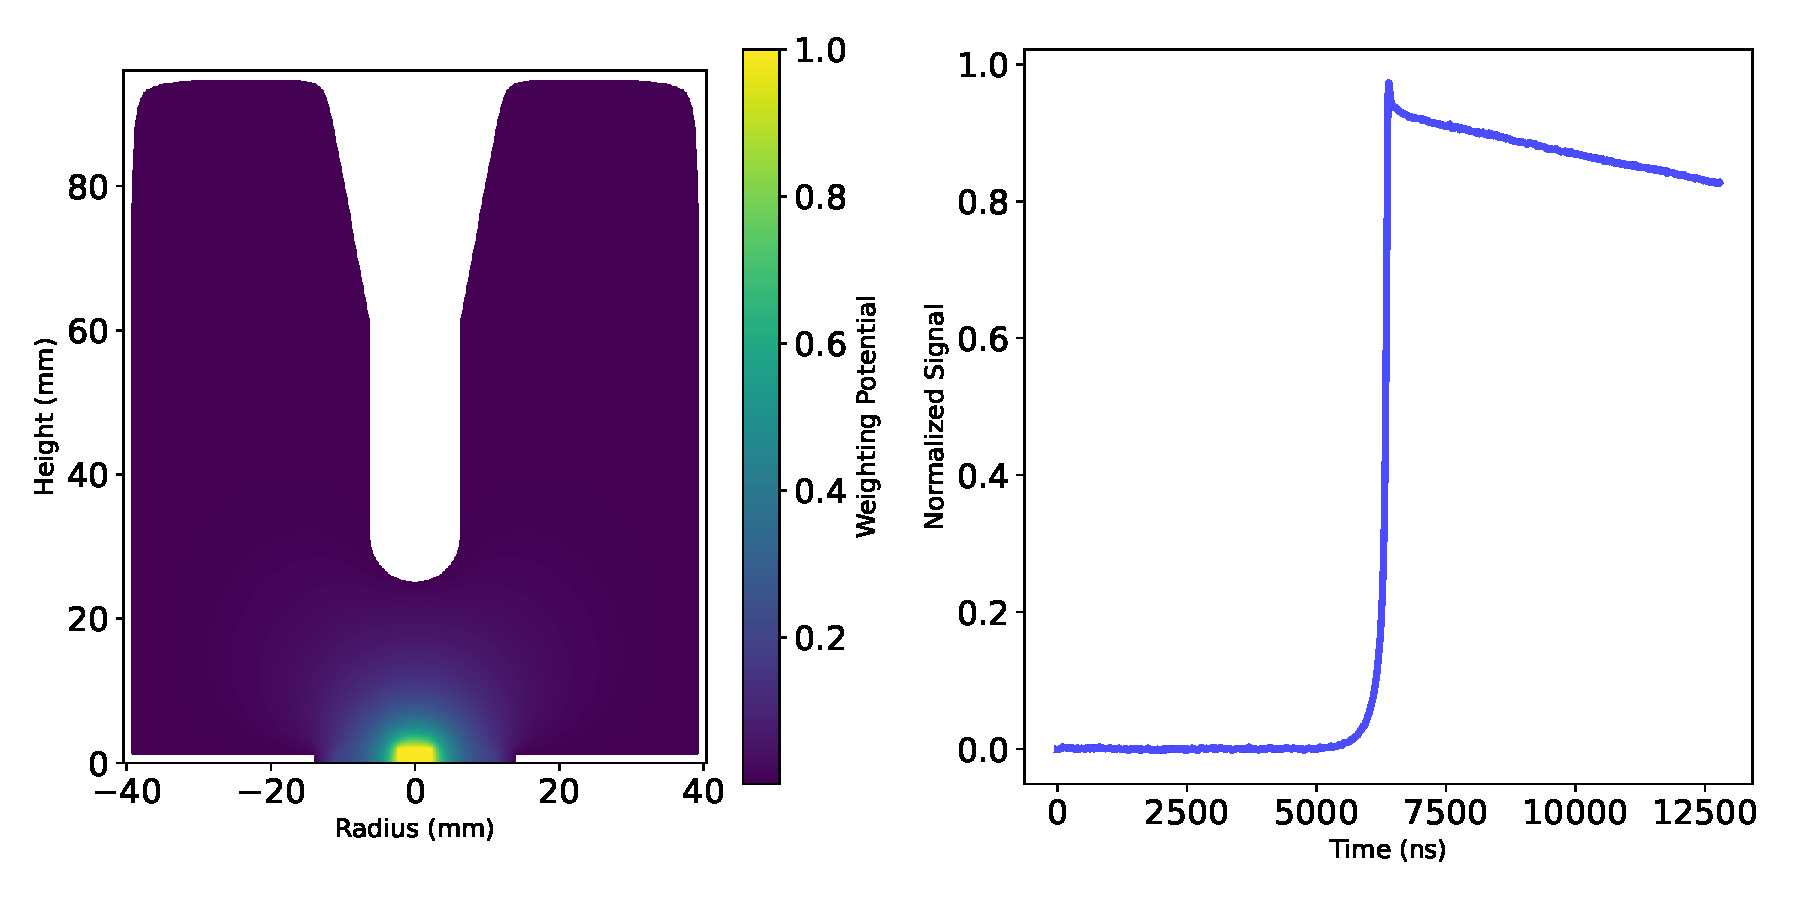
\includegraphics[trim=0 0.5cm 0 0,clip,width=\linewidth]{ch2/figs/wp_det.pdf}
  \caption{Left: Simulated weighting potential inside a LEGEND ICPC style point contact detector. Right: Collected signal from a detector showing sharp step shaped waveform.}
    \label{fig:wp_signal}
  \end{figure}

The pulse shape, along with long drift time and short collection time, provides an opportunity to veto multi-site events from gamma rays using analysis cuts. As the drift time varies with the path taken, multiple steps can often be identified in waveforms associated with multi-site events. The MAJORANA and GERDA collaborations are experiments with extensive experience in the research and development of Germanium detectors for {\onbb} searches.


\section{The MAJORANA DEMONSTRATOR}

The MAJORANA DEMONSTRATOR (MJD), located at the Sanford Underground Research Facility (SURF) in the USA, operated an array of 30 kg of enriched p-type, point-contact (PPC) detectors developed by ORTEC. The detectors were split between two vacuum-insulated cryostats housed within a low-background shield and operated in a vacuum at liquid nitrogen (LN) temperature, as shown in Fig. \ref{fig:mjd}. 

MJD pioneered the development of underground electroformed Copper (EFCu), where one obtains the purest Cu commercially available and electroforms it underground to reduce contamination from cosmogenically produced $^{60}$Co. This also lowered the concentration of natural $^{238}$U and $^{232}$Th contaminants by a factor of approximately 30 \cite{Abgrall:2016cct}. Another key innovation was the use of a low-mass front-end (LMFE) electronics board. The LMFE was designed to be highly radio-pure and hence reduced the background close to the detector. It also helped reduce noise in the signal as the first stage of amplification occurred very close to the detector. With its ultra-clean procedures, underground electroformed Copper and advances in front-end electronics, MJD achieved the lowest energy resolution in any large scale {\onbb} decay experiment of $2.52$keV ($0.12\%$) FWHM at $Q_{\beta\beta}$ when combining all detectors, and the second-lowest background index of $16.6^{+1.4}_{-1.3} \times 10^{-3} \text{ cts/(FWHM kg yr)}$ \cite{Majorana_final}.

\begin{figure}
  \centering
  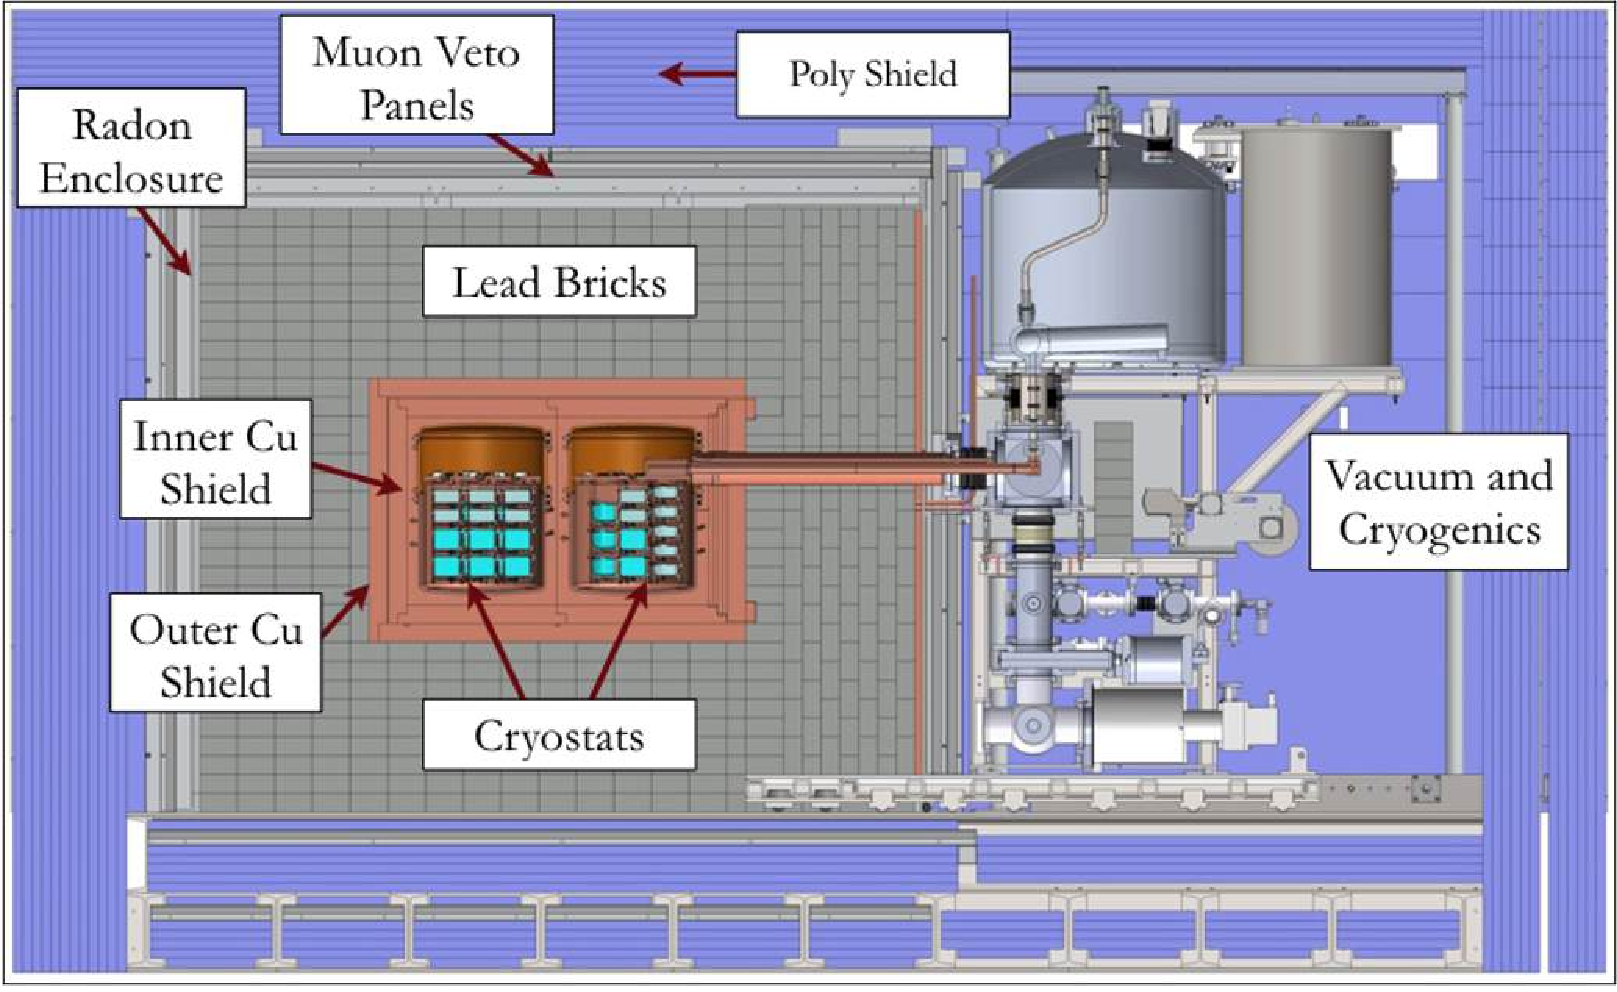
\includegraphics[height=0.34\columnwidth]{ch2/figs/mjd_setup.pdf}
  \qquad
  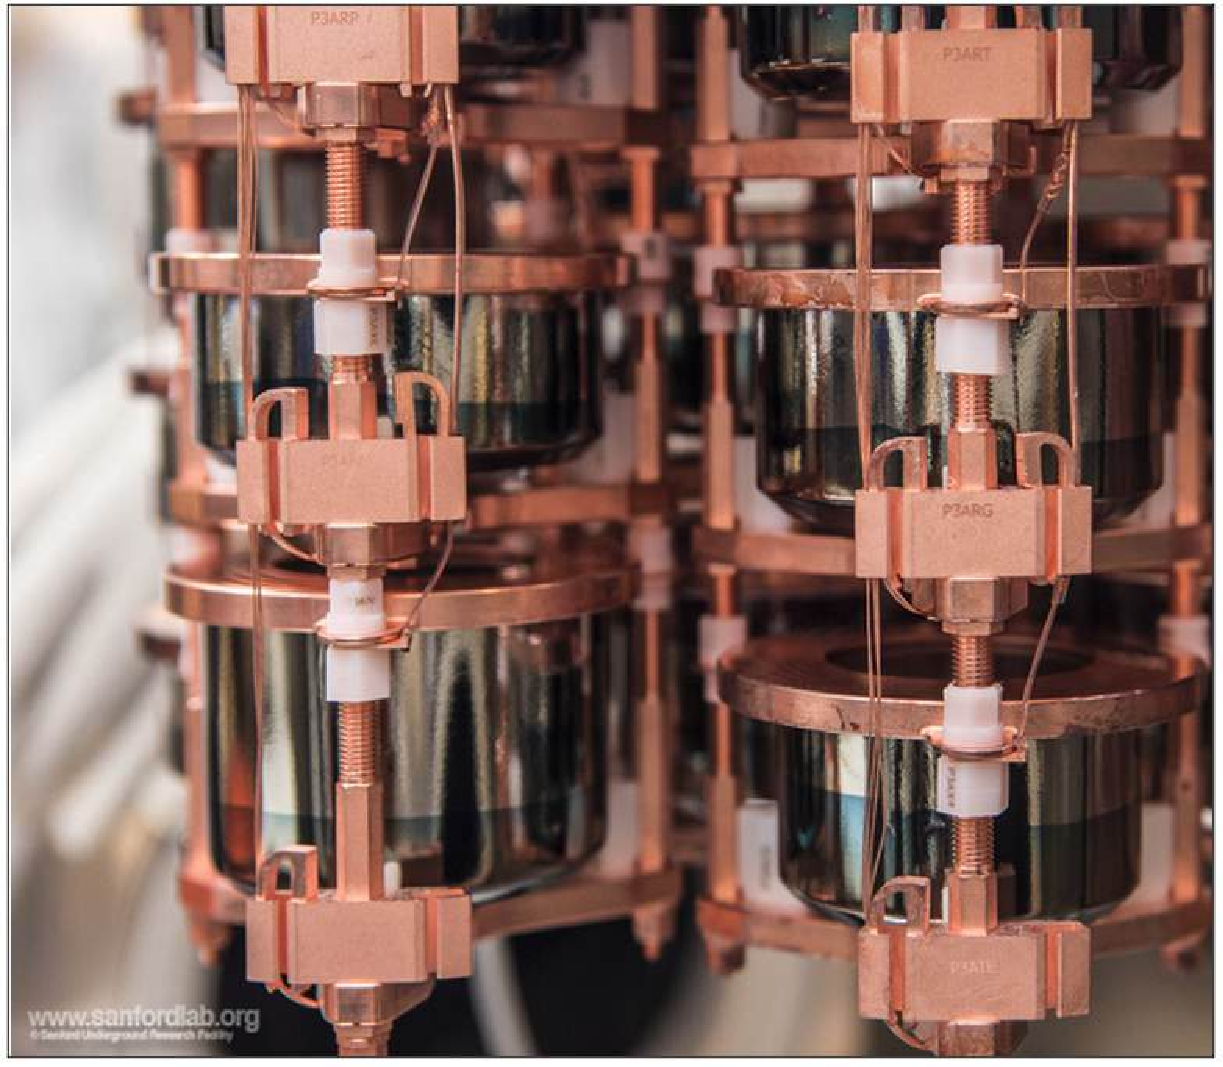
\includegraphics[height=0.34\columnwidth]{ch2/figs/mjd_ppc_array.pdf}
  \caption{The MAJORANA Demonstrator setup (left) and its Ge detector arrays (right).}
    \label{fig:mjd}
  \end{figure}
 
\section{The GERmanium Detector Array}

The GERmanium Detector Array (GERDA) collaboration was another enriched Germanium detector-based experiment, located at Laboratori Nazionali del Gran Sasso (LNGS) in Italy. GERDA consisted of an array of $20$ kg of enriched, customized versions of broad-energy Ge (BEGe) detectors and $15.6$ kg of enriched semi-coaxial detectors developed by Mirion, as shown in Fig. \ref{fig:gerda}. In its last year of data taking, GERDA deployed an additional $9.6$ kg of the novel p-type inverted-coaxial point-contact (ICPC) detectors to verify their technical maturity for future LEGEND experiments.

GERDA took a unique approach to reduce background: operating the detectors in liquid Argon. The detector strings submerged in liquid Argon were surrounded by a shroud of wavelength-shifting fibers, and the entire LAr cryostat was surrounded by water that enabled a muon veto using Cherenkov radiation. The fibers converted Ar $128$ nm scintillation photons into green photons, which were observed using silicon photomultipliers (SiPMs) attached to the ends of the fibers. This enabled a coincidence combining events detected in the Germanium detectors and the scintillation light read by SiPMs. The LAr veto allowed GERDA to distinguish gamma backgrounds from {\onbb} signal candidate events with high efficiency, achieving a background rate of $5.2^{+1.6}_{-1.3}\times 10^{-4}$ ct/(keV kg yr) and reached a half-life sensitivity above $10^{26}$ years \cite{GERDA_final}.

\begin{figure}
\centering
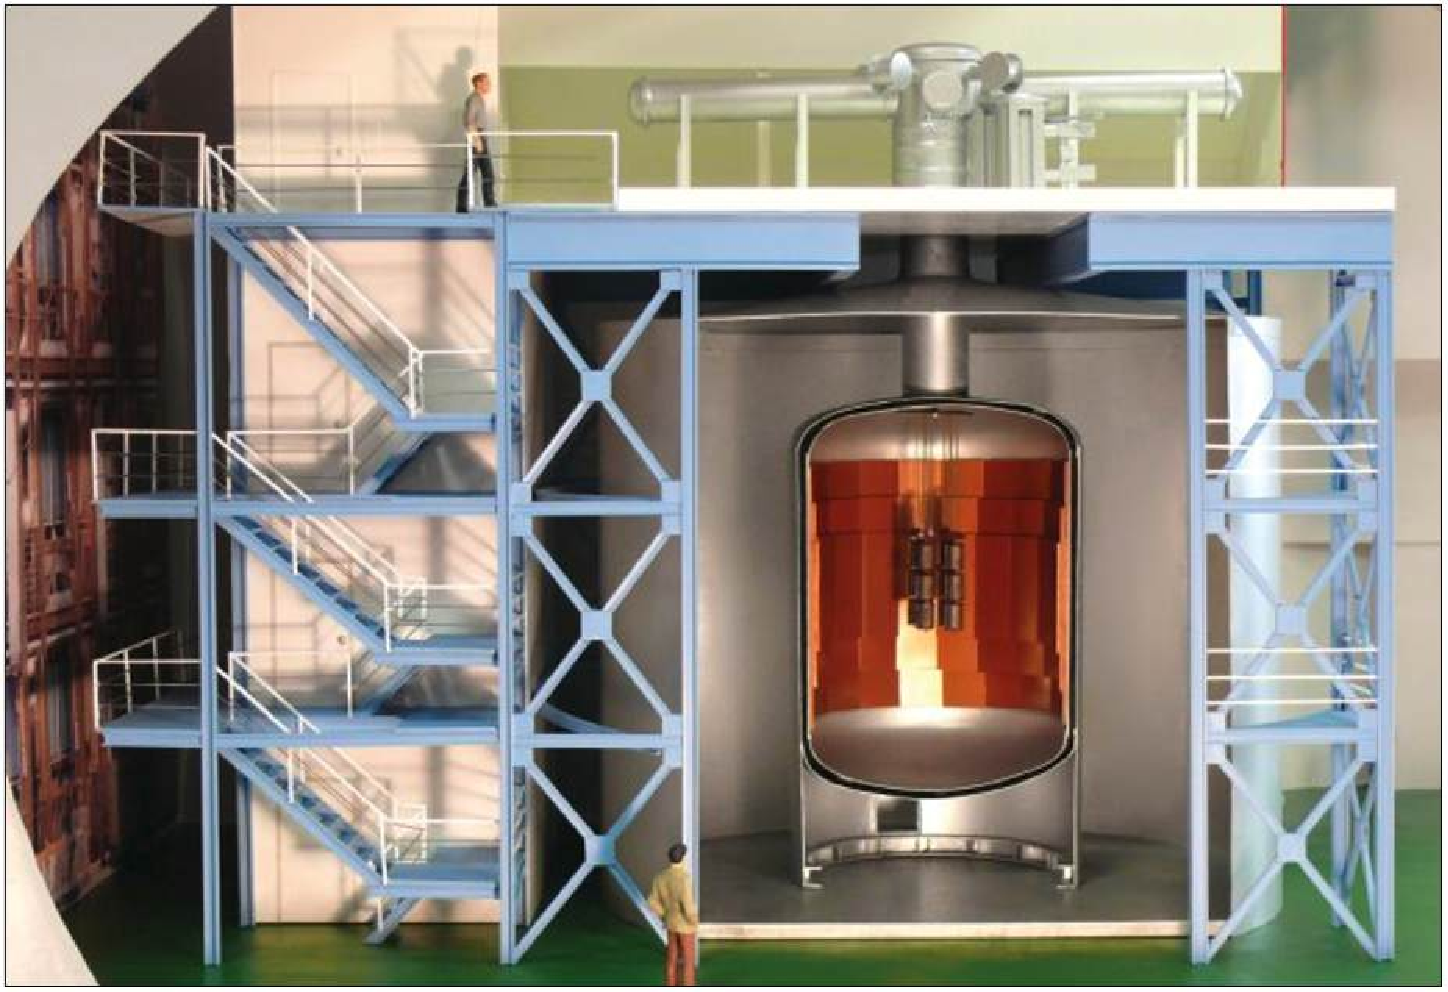
\includegraphics[height=0.385\columnwidth]{ch2/figs/gerda_setup.pdf}
\qquad
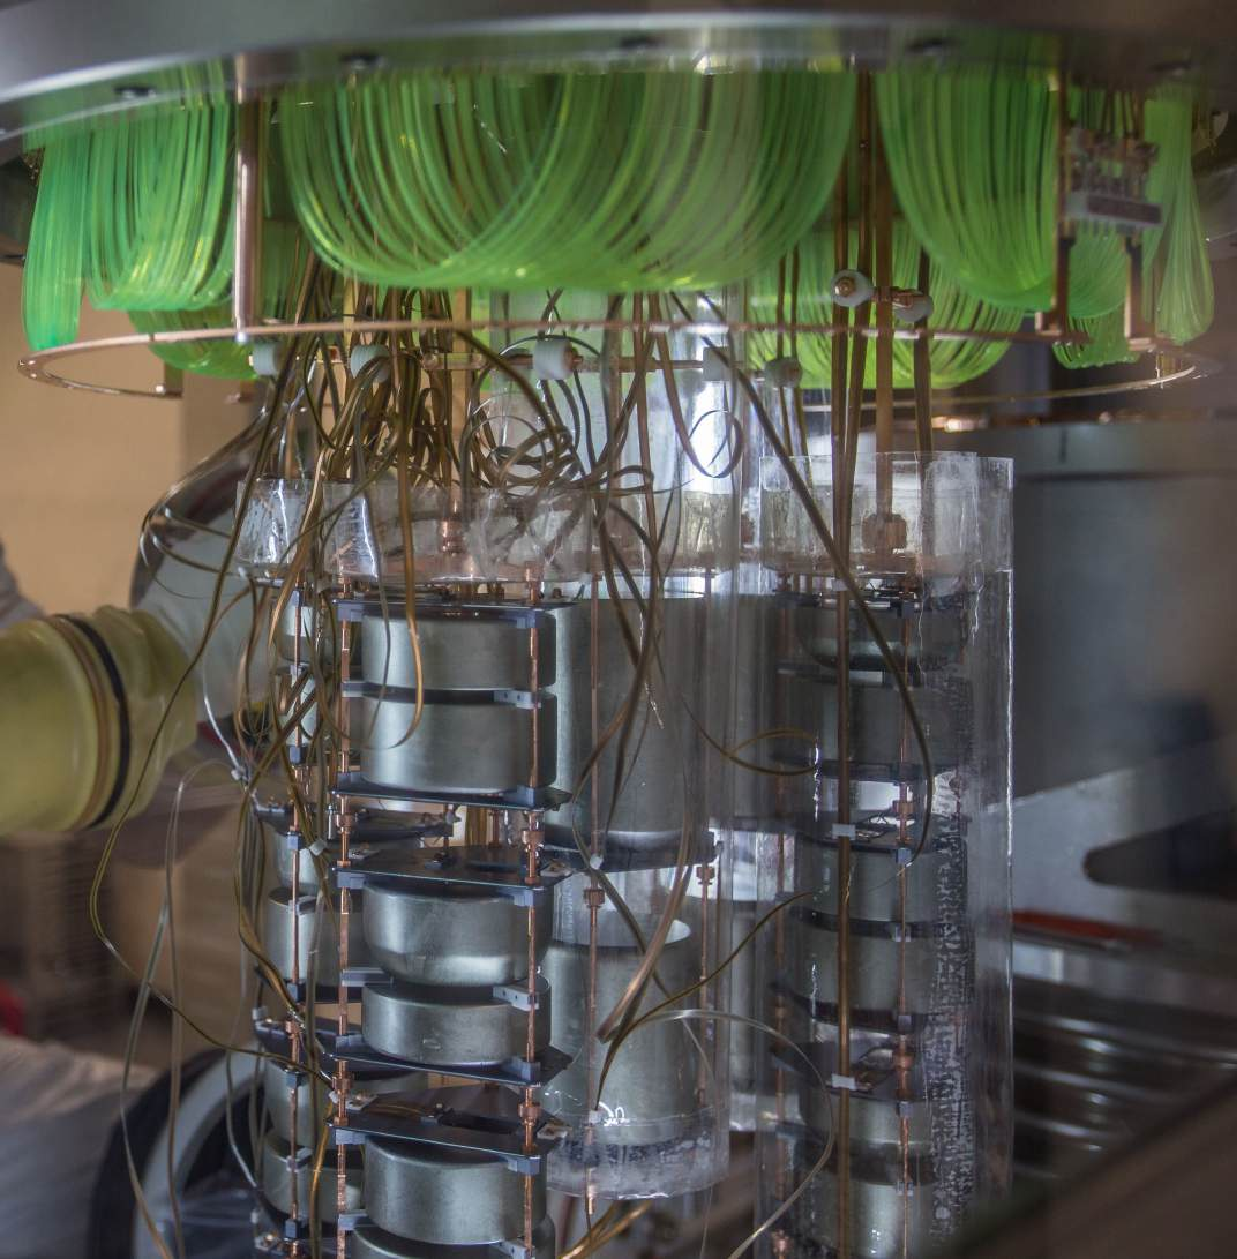
\includegraphics[height=0.385\columnwidth]{ch2/figs/gerdastrings.pdf}
\caption{GERDA setup (left) with Ge detectors (right) arranged in vertical strings.}
\label{fig:gerda}
\end{figure}
  
\section{The LEGEND experiment}
The Large Enriched Germanium Experiment for Neutrinoless $\beta\beta$ Decay (LEGEND) is a next-generation experiment that combines the best techniques and resources from GERDA and MJD. In both previous experiments, the maximum mass of the detectors was constrained by electrode geometry to $1$ kg. Higher mass results in a lower surface-to-volume ratio and thus reduces the per-channel background, as well as decreases the number of channels needed, reducing per-kg background from cables, connectors, and detector mounts. A major innovation for LEGEND has been the development of p-type inverted-coaxial point-contact (ICPC) detectors, which can be manufactured with masses of around $2-3$ kg. LEGEND is taking a phased approach to a double-beta decay experimental program.

\subsection{LEGEND-200}

The first phase currently underway consists of 200 kg of Germanium detectors housed in an upgrade of the GERDA infrastructure at LNGS. Enriched PPC and BeGe detectors from MJD and GERDA will make up 70 kg of the source mass, and the newly-manufactured ICPC detectors will make up the rest of the 130 kg. The setup is illustrated in Fig. \ref{fig:L200}. 

MJD achieved excellent energy resolution, primarily due to its low noise and low background electronics. Background model spectral fits indicated that the dominant source of background in MJD was not from $^{208}$Tl sources close to the detectors. \cite{Buuck_thesis}. On the other hand, GERDA achieved a very low background index with the help of its efficient LAr veto. Prominent features from its background model were from $^{210}$Po on the surface of the Ge-detector p$^+$ electrode, $^{232}$Th and $^{238}$U decay chains, and $^{42}$Ar progeny. GERDA's background model fits suggest that the dominant background contributions \cite{GERDA_final} were from components close to the detector array.

{\Ltwo} inherits the best of both experiments. It uses MJD's low background materials and electronics to counter the background GERDA faced close to the detector and uses a LAr veto with improved scintillation light readout to reduce the distance-component backgrounds faced by MJD. The introduction of ICPC detectors also results in a lower surface-to-volume ratio, allowing for a reduction of the net radioactive $\alpha$ and $\beta$ decays near the surface. Higher mass detectors also decrease the need for detector support materials and electronics that can be a source of background. 

\begin{figure}[!htb]
 \centering
 %[trim={left bottom right top},clip]
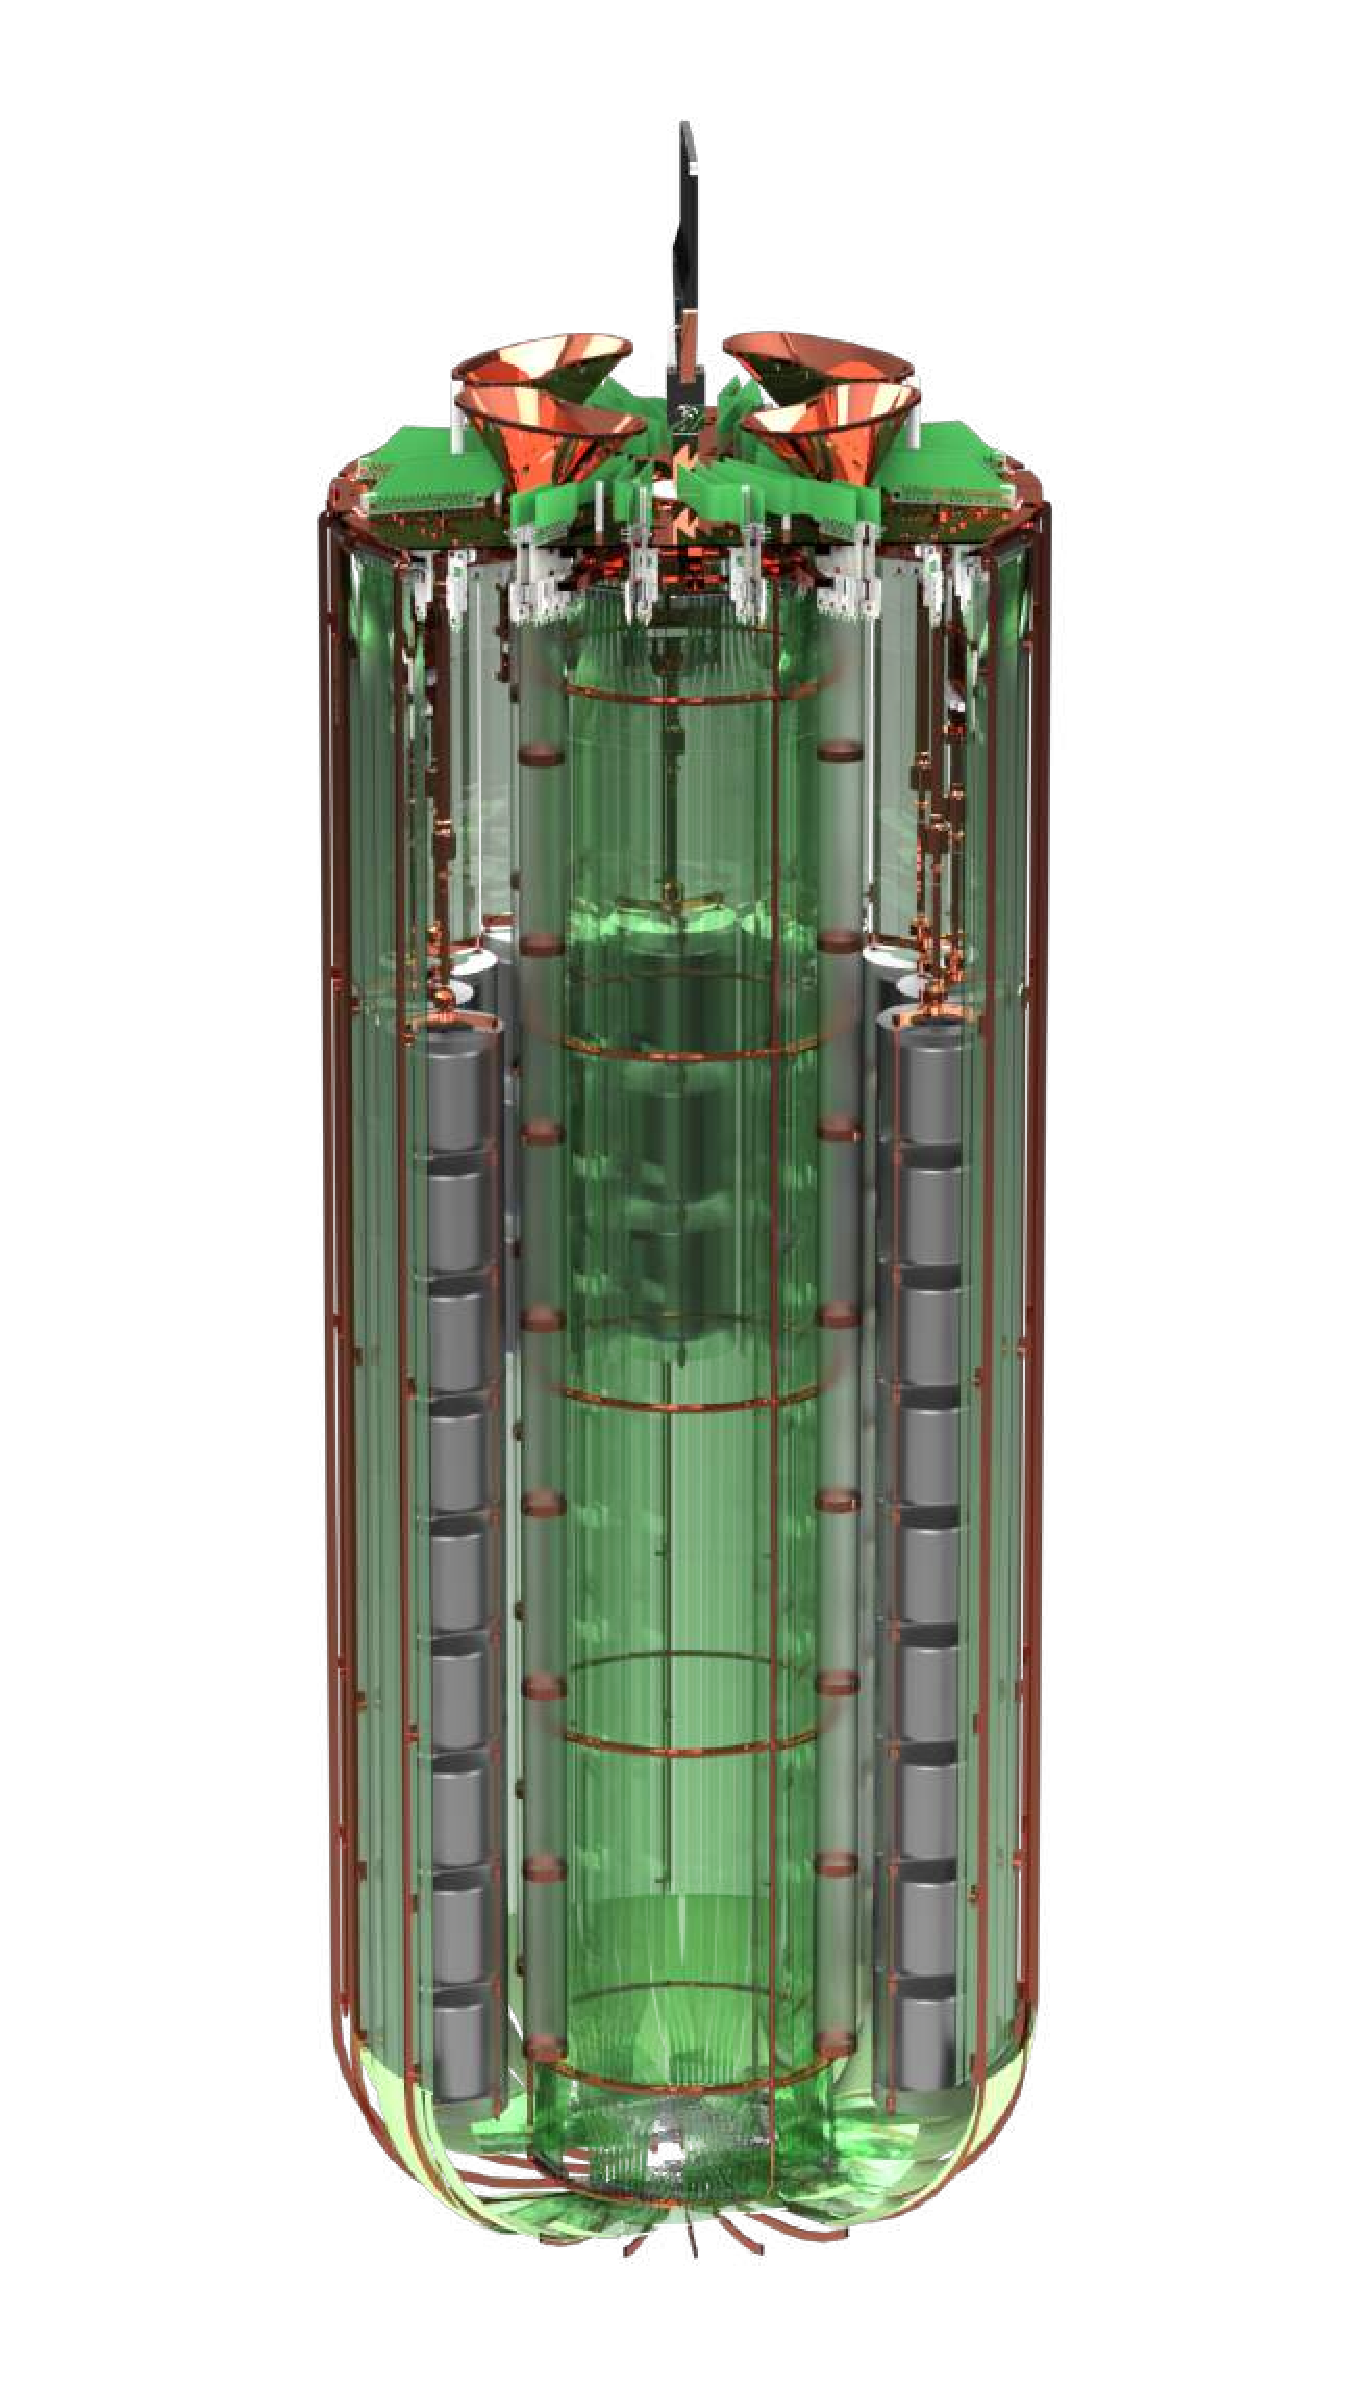
\includegraphics[trim=0 1cm 0 0,clip,height=0.4\linewidth]{ch2/figs/l200_strings.pdf}
\qquad
  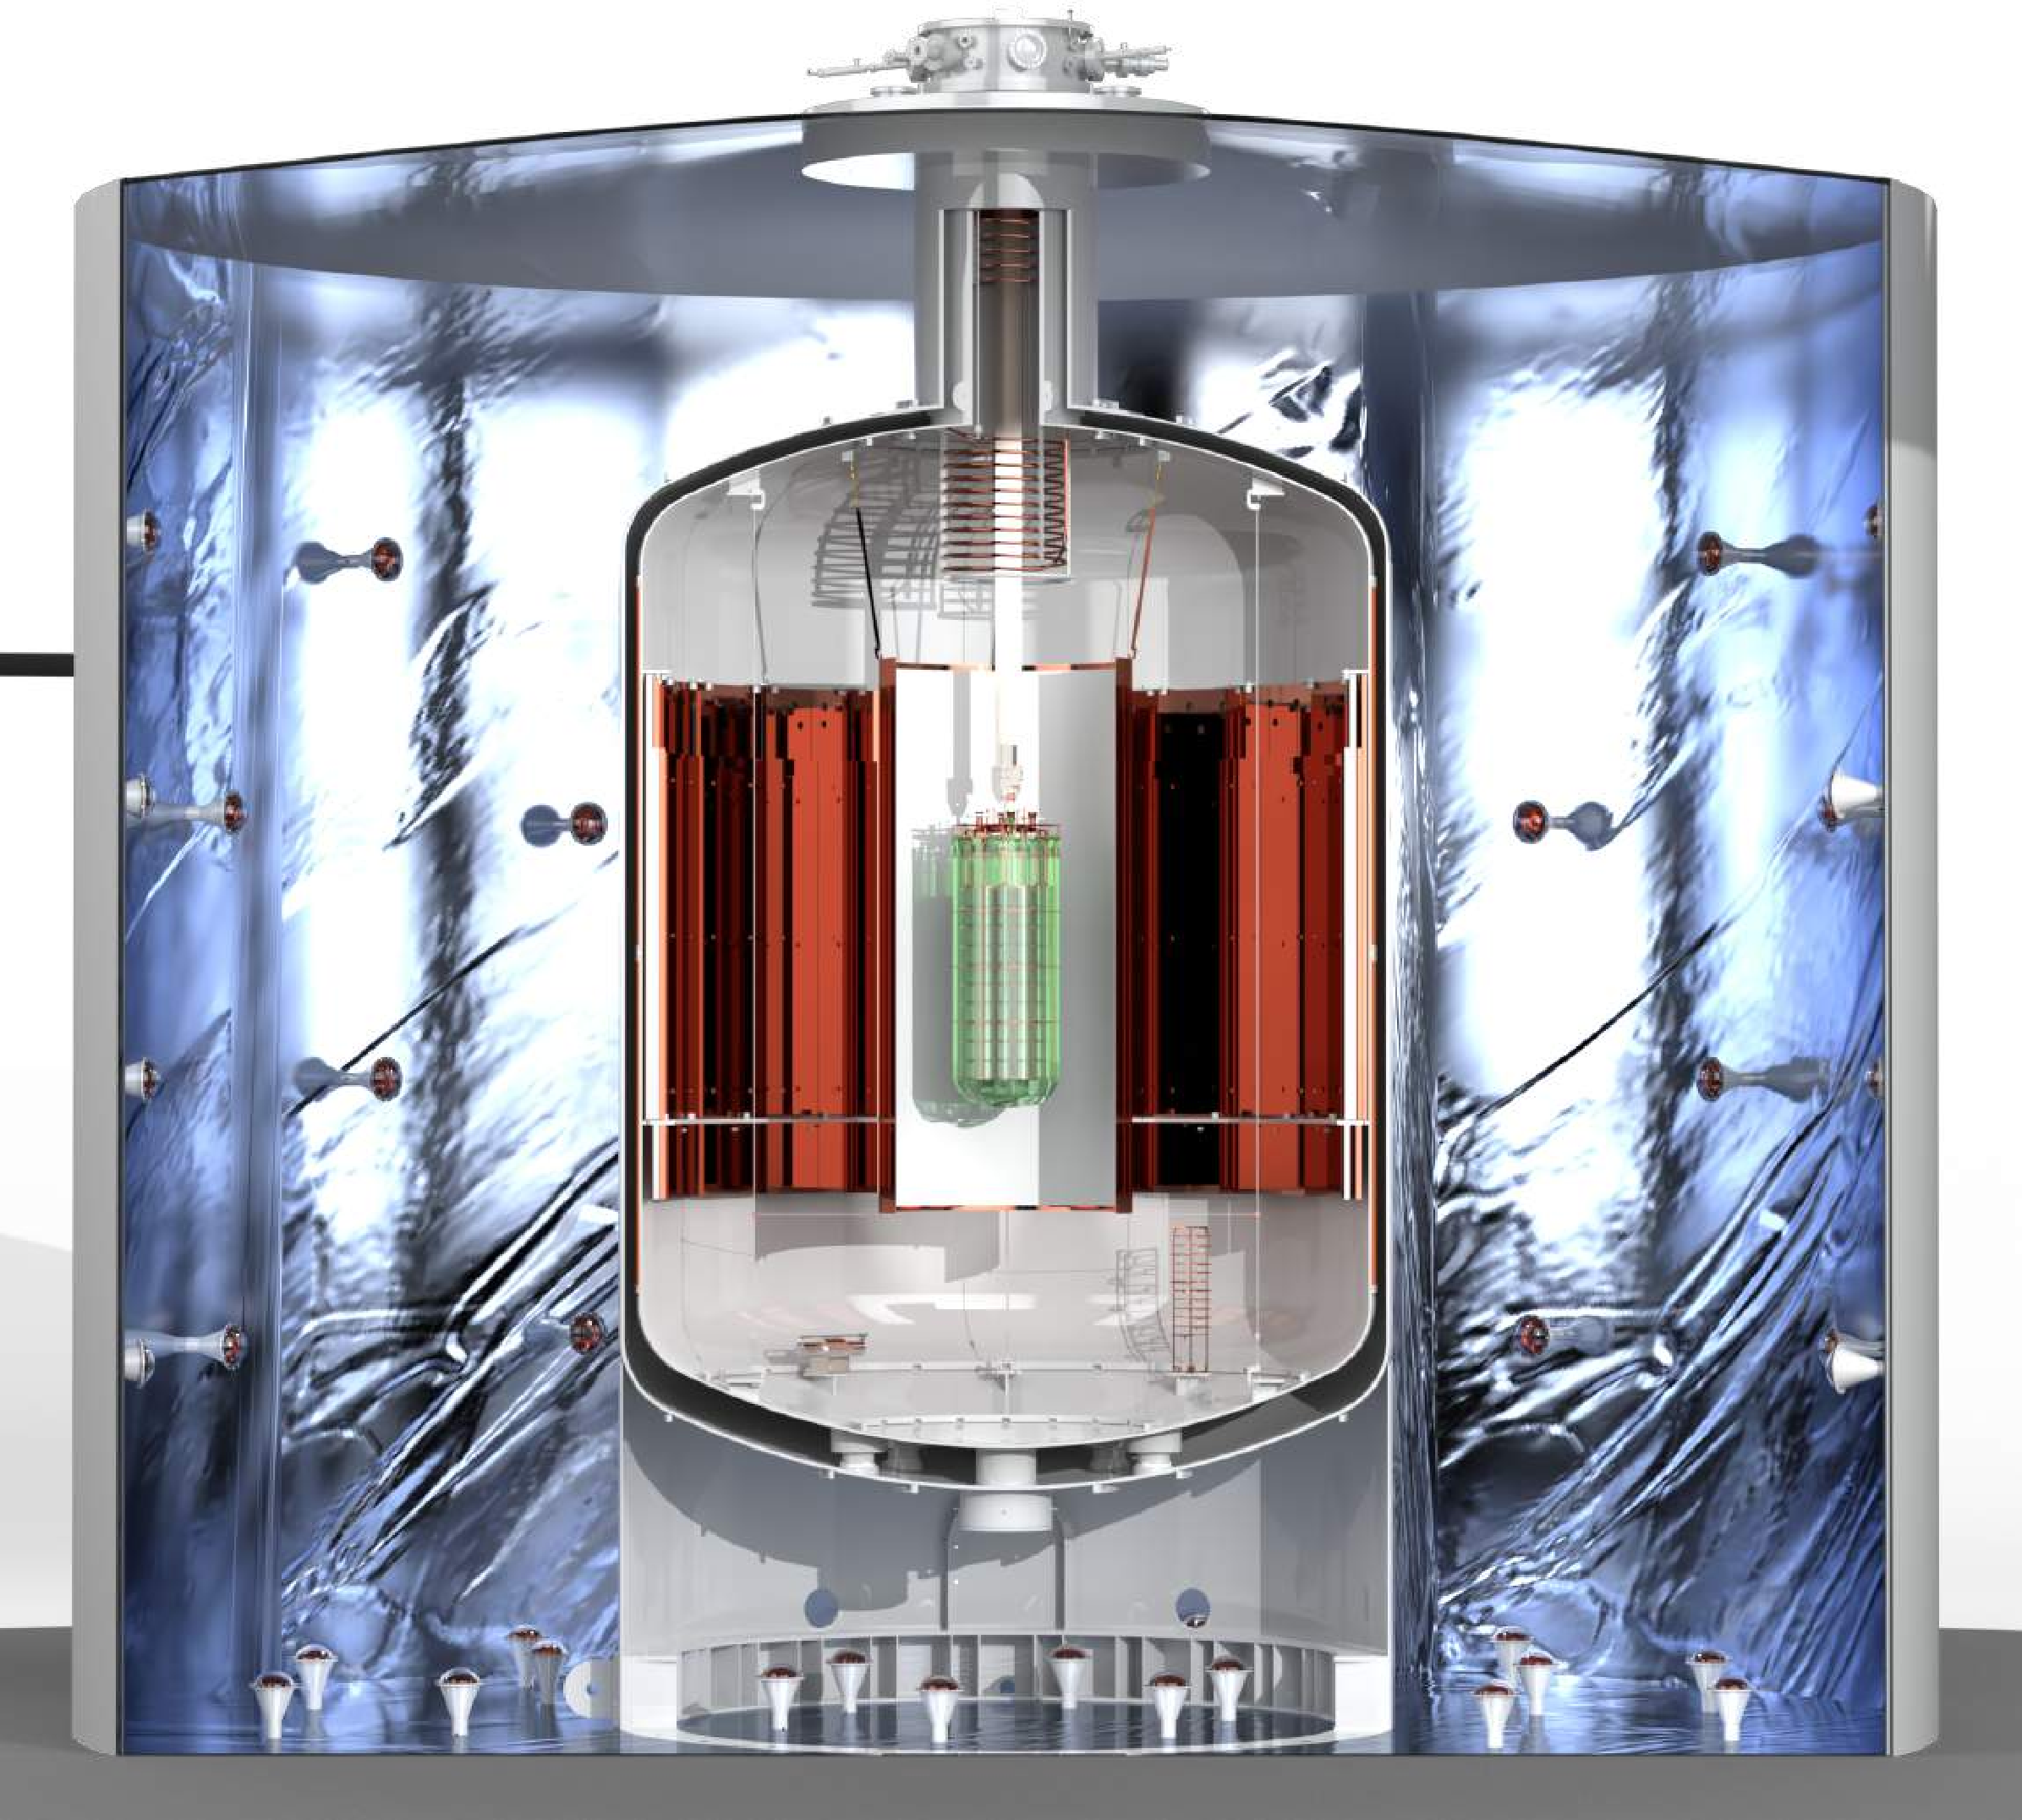
\includegraphics[height=0.4\linewidth]{ch2/figs/l200_fig.pdf}
 \caption{\label{fig:L200} Left: {\Ltwo} Ge detectors strings
 surrounded by wavelength-shifting fibers for LAr veto. Right: The L-200 design. The detector array is mounted in the center of the LAr cryostat. Muon veto is achieved by placing the cryostat in a water tank and detecting Cerenkov radiation with photo-multipliers. %\cite{l1000_pcdr} (Picture courtesy P. Krause).
}
\end{figure}

\begin{figure}[!htb]
  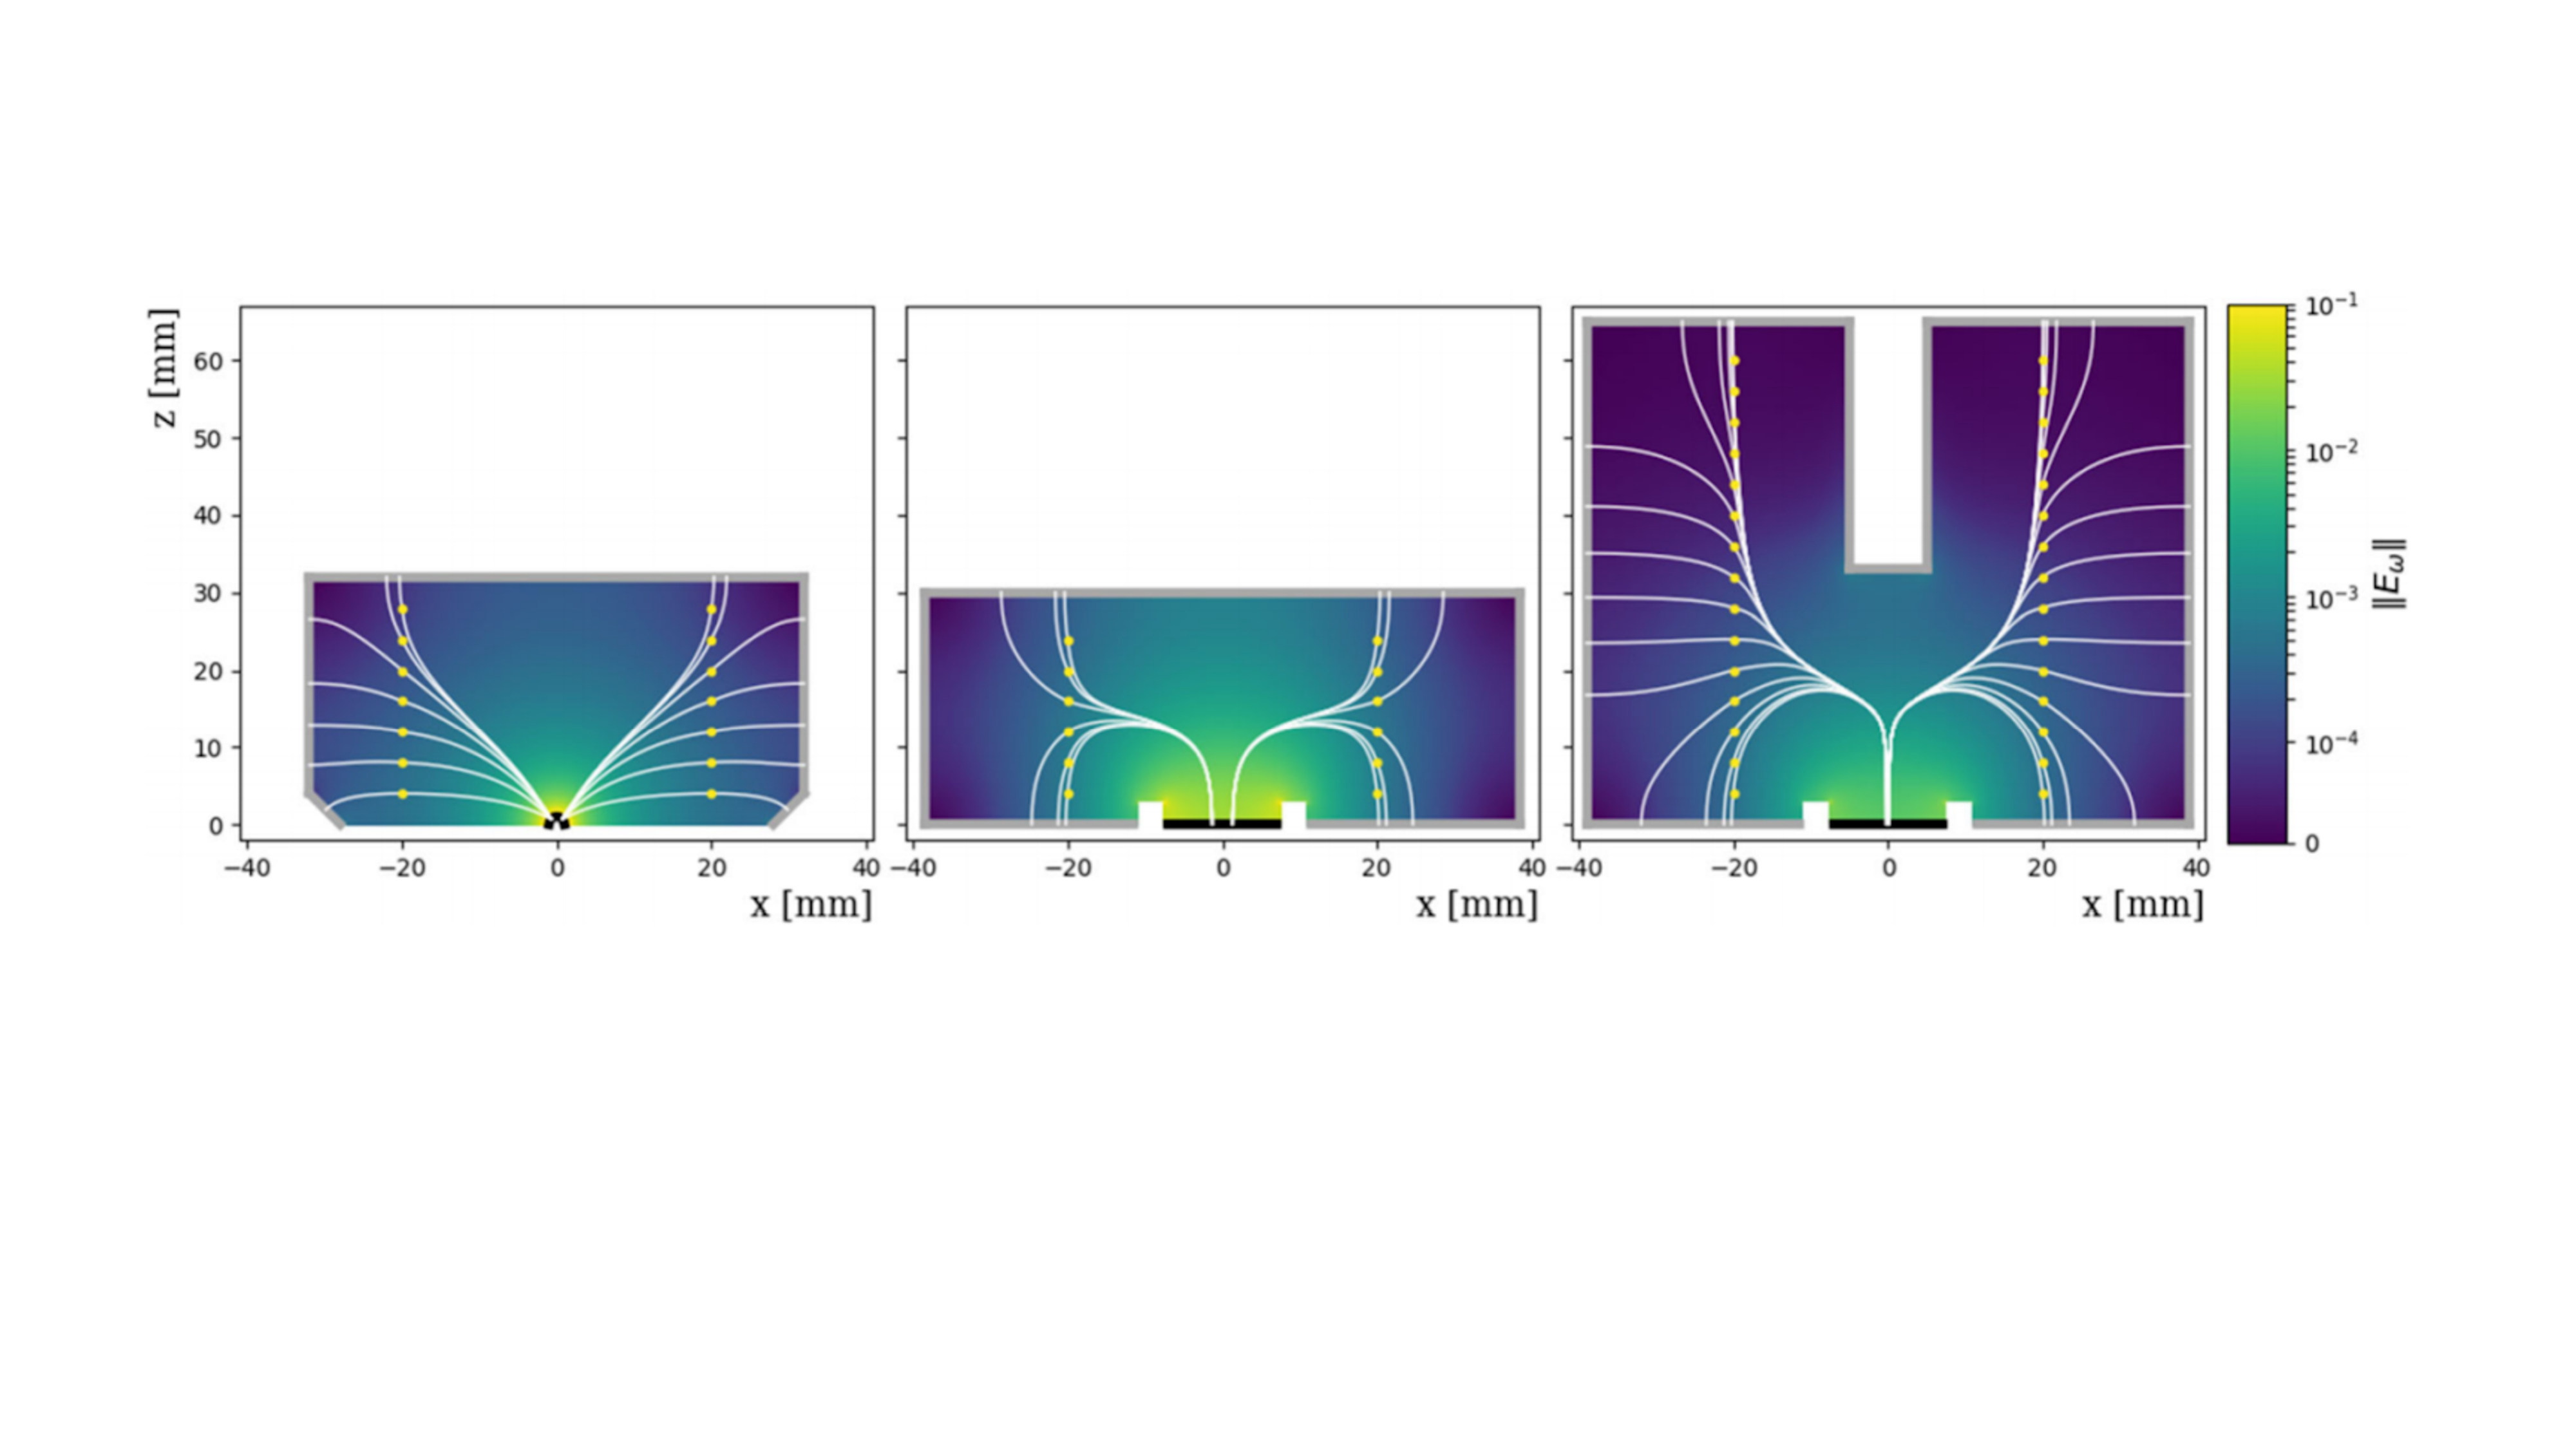
\includegraphics[trim=15 30 15 20,clip,width=\linewidth]{ch2/figs/Det-geo-2.pdf}
\caption{The three detector geometries used in LEGEND: {\MJD} PPC detectors (left), GERDA BEGe detectors (middle), and newly developed ICPC detectors (right).The plots depict the weighting field ($E_\omega$) within each detector's cross section.The thick black and gray lines are the p$^+$ and n$^+$ electrode, respectively. The yellow points are locations of simulated energy depositions. The holes travel along the white lines to the p$^+$ electrode, while electrons travel along the while line to the n$^+$ electrode. Figure from \cite{Comellato:2020ljj}.}
\label{fig:det-compare}
  \end{figure}
  
The three kinds of detector geometries that LEGEND uses are illustrated in Fig. \ref{fig:det-compare}. The p$^+$ contact is created using Boron implantation at the crystal end with the highest impurity. The n$^+$ region is created using the diffusion of Lithium atoms onto the detector surface. To isolate the two electrodes from each other, the surface region in between is passivated, usually with amorphous germanium. The electric field is carefully designed by controlling the impurity gradient in the bulk of the crystal. 


{\Ltwo} began with a 142 kg source configuration from March of 2023 until February of 2024. The first data was unblinded on June 13, 2024. After applying analysis cuts, a total of seven events were observed in the region of interest, corresponding to a background index of $ (5.3 \pm 2.2) \times 10^{-4} \text{ cts/(keV$\cdot$kg$\cdot$yr)}$. A combined fit incorporating results from GERDA, MAJORANA, and LEGEND-200 yielded a background-only $p$-value of 26\%, indicating no significant excess over expected background. The lower limit on the 0$\nu\beta\beta$ half-life was set at $T^{0\nu}_{1/2} > 1.9 \times 10^{26} \text{ yr} \quad \text{(90\% C.L.)}$ with an expected sensitivity of $2.8 \times 10^{26}$ years. \cite{Pertoldi2024}

\subsection{LEGEND-1000}
The subsequent phase of LEGEND is a proposed ton-scale experiment. A ton-scale experiment will probe the entire inverted ordering mass hierarchy, with the capability to make an unambiguous discovery of {\onbb} with $3\sigma$ certainty. It would also cover half of the normal ordering parameter space, under certain assumptions \cite{l1000_pcdr}. LEGEND-1000 builds upon the innovation and research done in {\Ltwo}. It will use ICPC detectors that have demonstrated lower surface backgrounds, excellent energy resolution, and precise pulse shape discrimination. The experiment also plans to use underground-sourced liquid Ar, which would greatly reduce the $^{42}$Ar background. LEGEND-1000 would probe a half-life of $10^{28}$ years, which corresponds to $m_{\beta\beta}$ range of $9$-$21$ MeV after 10 yr of data taking. The Pre-Conceptual Design Report for LEGEND-1000, with a detailed design description and information about the discovery potential, can be found at \cite{l1000_pcdr}. {\Ltwo} will be the main scope of this thesis, with the goal of developing techniques towards {\Lthou}.


%\subsection{Pulse Shape Discrimination}


\section{{\Ltwo} background model}

{\Ltwo} has very low backgrounds. Fig. \ref{fig:L200_background} shows the expected background contribution in {\Ltwo}. These components are calculated using radiopurity assays of selected materials and Monte Carlo simulations. 

\begin{figure}[!htb]
\centering
  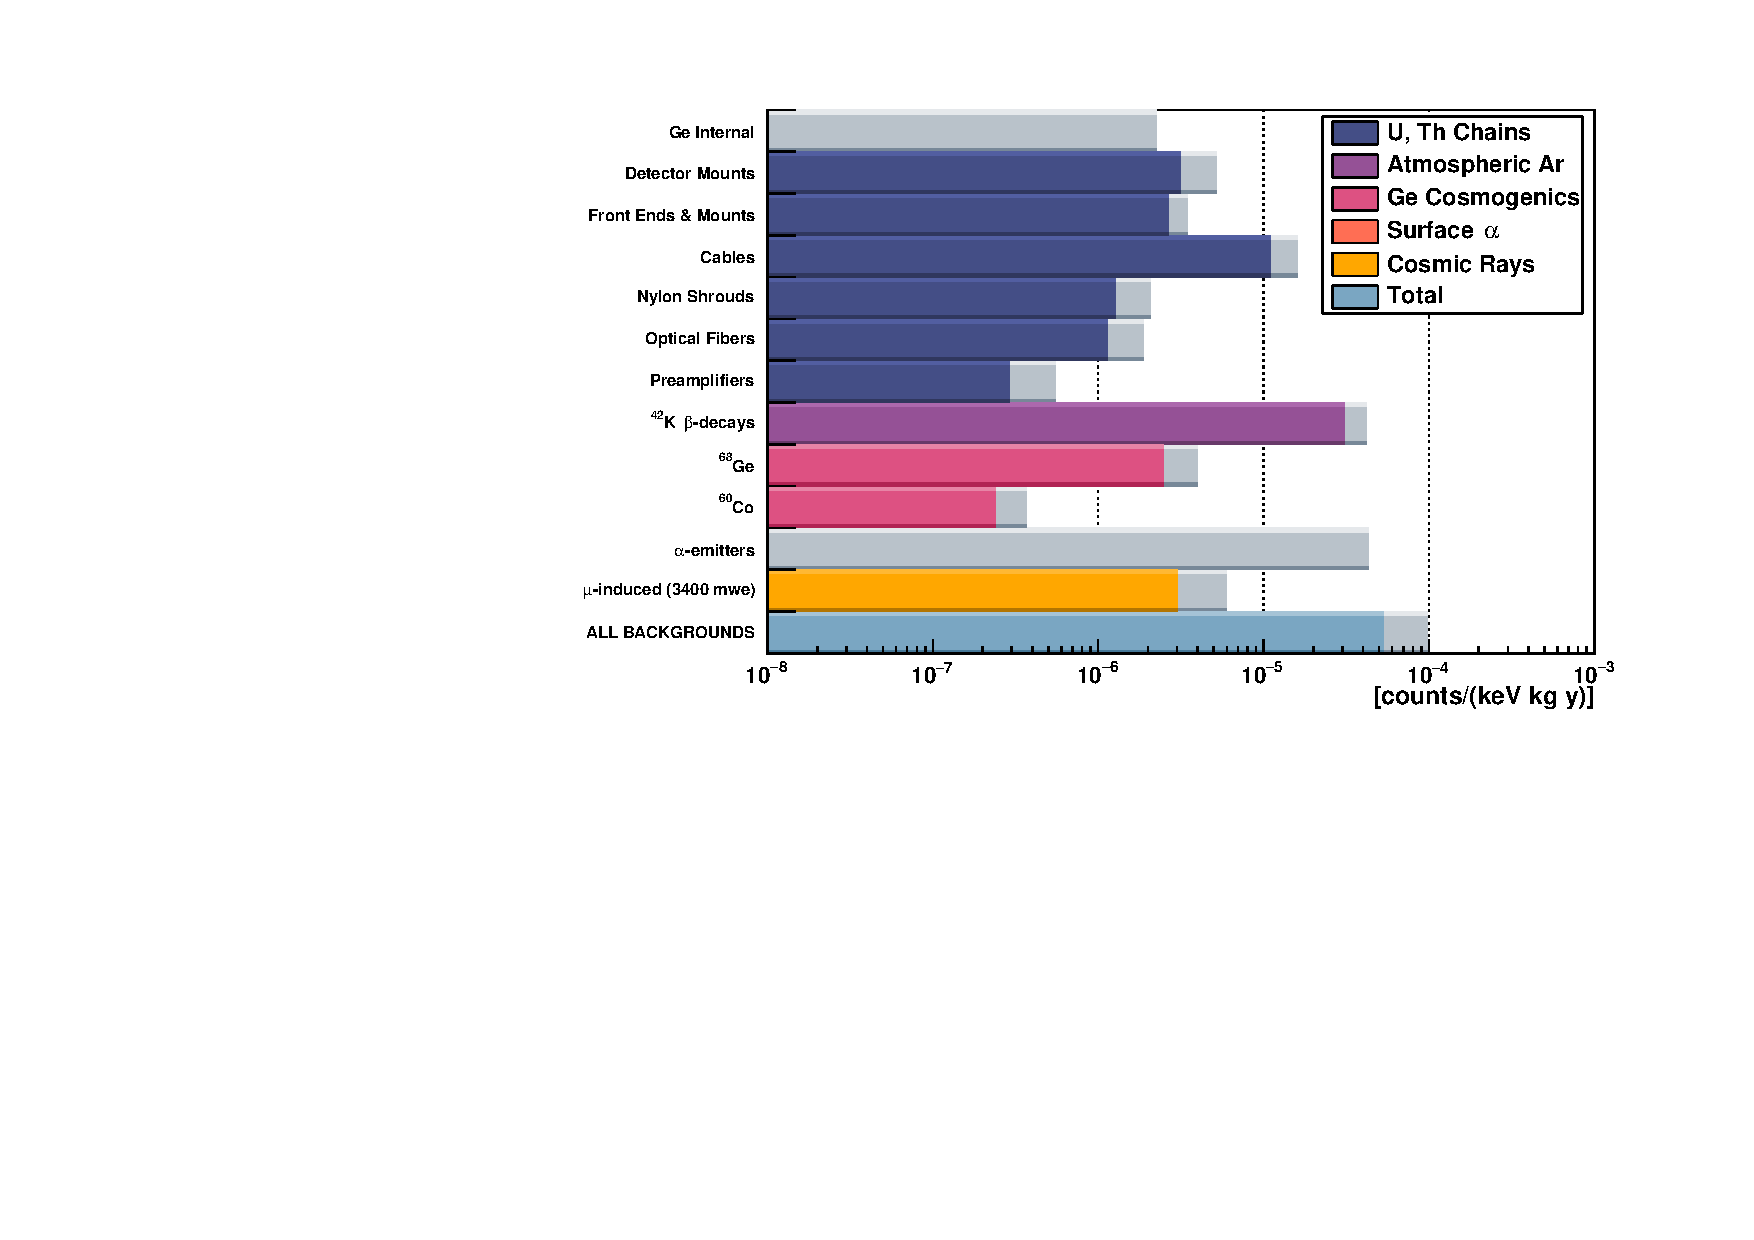
\includegraphics[width=0.8\linewidth]{ch2/figs/L200_background.pdf}
  \caption{{\Ltwo} Projected background contributions near Q$_{\beta\beta}$ after all analysis cuts. Grey bands indicate uncertainties in assays and background rejection.}
\label{fig:L200_background}
  \end{figure}


  
Decays of long-lived $^{238}$U and $^{232}$Th isotopes, as well as their short-lived progeny, are major backgrounds from component materials. They are primarily reduced by using higher purity materials and reducing materials close to the detectors. Cosmogenic backgrounds $^{68}$Ge and $^{60}$Co isotopes are produced when Ge is exposed to neutrons produced by cosmic rays. This background can be reduced by controlling the cosmic-ray exposure during the production and increasing the underground cool-down period for the experiment. 

Surface events such as alphas and $^{42}$K betas are one of the biggest contributions to the background. The use of liquid Argon introduces two short-lived isotopes, $^{39}$Ar and $^{42}$Ar.  $^{42}$Ar decays into $^{42}$K which is positively charged and can drift with the applied electric field to the detector surface. It can then undergo a $\beta$ decay with a Q value of $3525$ keV overlapping with the region of interest. $^{42}$Ar is formed by cosmogenic exposure of atmospheric Ar, and the best way to mitigate its background is to use underground-sourced liquid Argon as in LEGEND-1000.

Alpha backgrounds come primarily from surface contaminants such as $^{210}$Po and $^{210}$Pb, introduced as dust during fabrication, storage, and assembly processes, or through depositions of the ionized progeny of $^{222}$Rn decays. Alpha backgrounds can be reduced by handling the detectors and surrounding materials with care in ultra-clean, inert environments. In LEGEND, support materials are etched using acids or leached in Nitric acid to reduce radon implantation, and then the detectors are assembled and installed into cryostats using a glove box with a radon-reduced dry Nitrogen environment. The use of liquid Argon reduces the alpha background due to gaseous $^{222}$Rn previously observed in MJD.



\begin{figure}
\centering
  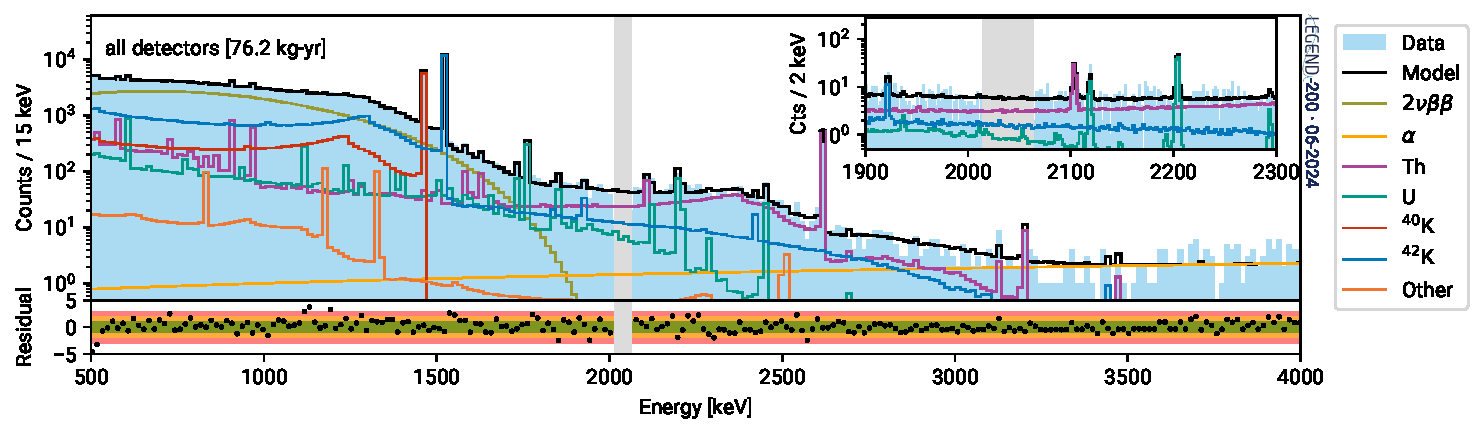
\includegraphics[width=0.99\linewidth]{ch2/figs/l200-bkgmodel-2_compressed.pdf}
  \caption{{\Ltwo} background contributions near Q$_{\beta\beta}$ after all analysis cuts. Credit: Toby Dixon, Luigi Pertoldi}
\label{ch2:fig:L200_background_model_fit}
  \end{figure}

  

 The alpha background contribution in Fig. \ref{fig:L200_background} has a  high uncertainty. These uncertainties are driven by uncertainty in the pulse shape rejection for background components. Pulse shape analysis can be used to reject background events coming from the passivated surface very efficiently; however, the effectiveness of those cuts is hard to model. This is because we don't have a good background component for alphas. Fig. \ref{ch2:fig:L200_background_model_fit} shows the background model in LEGEND-200. It is constructed using a global binned likelihood fit using measured spectra, radio assay data, Monte Carlo simulations, and special background runs. The model accurately describes gamma-induced backgrounds, but the alpha background component is mostly flat and remains poorly constrained due to modeling challenges. In the next chapter, we focus on understanding the surface backgrounds and introduce an approach that can help model their backgrounds.

% To conclude, HPGe provides a compelling approach to look for neutrinoless double beta decay. The signal formation is very well understood and can be modeled using simulations. LEGEND collaboration is looking for {\onbb} in Ge-76 using a phased approach and with a goal to probe the bottom of the inverted hierarchy. Surface backgrounds are the largest components in the background model and a significant source of uncertainty due to the lack of proper modeling. 